\documentclass[12pt]{beamer}
\usepackage[utf8]{inputenc}
\usepackage[T1]{fontenc}
\usepackage[portuguese]{babel}
\usepackage{amsmath}
\usepackage{amsfonts}
\usepackage{amssymb}
\usepackage{graphicx}
\usepackage{textpos}

\usetheme{Dresden}
\usecolortheme{beaver}

\makeatletter
\newlength\beamerleftmargin
\setlength\beamerleftmargin{\Gm@lmargin}
\makeatother

\begin{document}
	\author{
		André Correia Bueno \and
		Gabriel Petrini		\\\and
		João Paulo Farias Fenelon \and
		João Victor Machado
	}
	\title{Nelson e Winter (1982: cap 12): Dynamic Competition and Technical
		Progress}
	\subtitle{Competição dinâmica e progresso tecnológico}
	\institute{IE/Unicamp}
	\date{28 de Abril de 2020}
	\subject{OIDT}
	%\setbeamercovered{transparent}
	%\setbeamertemplate{navigation symbols}{}



\begin{frame}[plain]
	\maketitle
\end{frame}

\begin{frame}
\frametitle{Estrutura da Apresentação}
\tableofcontents
\end{frame}

\section{Introdução}

\begin{frame}
\frametitle{Introdução}
\begin{alert}{Objetivo}
	Analisar as relações entre estrutura de mercado e progresso tecnológico com desempenho industrial
\end{alert}


\begin{alert}{Por que uma abordagem evolucionária?}

\end{alert}

\end{frame}

\section{Fundamentação teórica}

\section{Modelo}

\begin{frame}
\frametitle{Overview}
\begin{alert}{Destaques (\textit{Science-based})}
	Uma firma pode reduzir seus custos unitários ao descobrir técnicas mais produtivas por meio de:
	
	\begin{itemize}
		\item Inovação
		\item Imitação
	\end{itemize}
	
	Ambas estratégias dependem do tamanho da firma ($K_{it}$), afetam a lucratividade ($\pi_{it}$) e são incertas ($Pr$). 
\end{alert}

\textbf{Resultado:} Estrutura de mercado é \textbf{endógena}
\end{frame}


\begin{frame}
\frametitle{Equações}

\[ \begin{array}{lrl}
\mbox{Plena Capacidade:} & Q_{i,t} = &A_{i,t}K_t\\
\mbox{Produto total:} & Q_t=  &\sum{Q_{i,t}}\\
\mbox{Curva de demanda:} & P =  & D(Q_t) \\
\mbox{Taxa de Lucro:} & \pi_{i,t} =& P_tA_{i,t} -c -r_{im} - r_{in}\\
\mbox{Sucesso imitação:} & Pr(d_{im}=1) =& a_mr_{im}K_{i,t} \\
\mbox{Sucesso inovação:} & Pr(d_{in}=1) =& a_nr_{in}K_{i,t} \\
\mbox{Mudança produtiva:} & A_{t+1} =& \max(A_{i,t}, \hat{A}_{t}, A^{\sim}_{i,t}) \\
\mbox{Expansão:} & \Delta K_{t+1} =& I(\mu, s, \pi_{i,t}, \delta)\cdot K_{i,t} -\delta K_{i,t}\\
\mbox{Reprodução simples:} &\lim_{s\to0} & I(1,s,0,\delta)  = \delta \\
\end{array}\] 
\end{frame}

\begin{frame}[plain]
\hspace*{-\beamerleftmargin}%
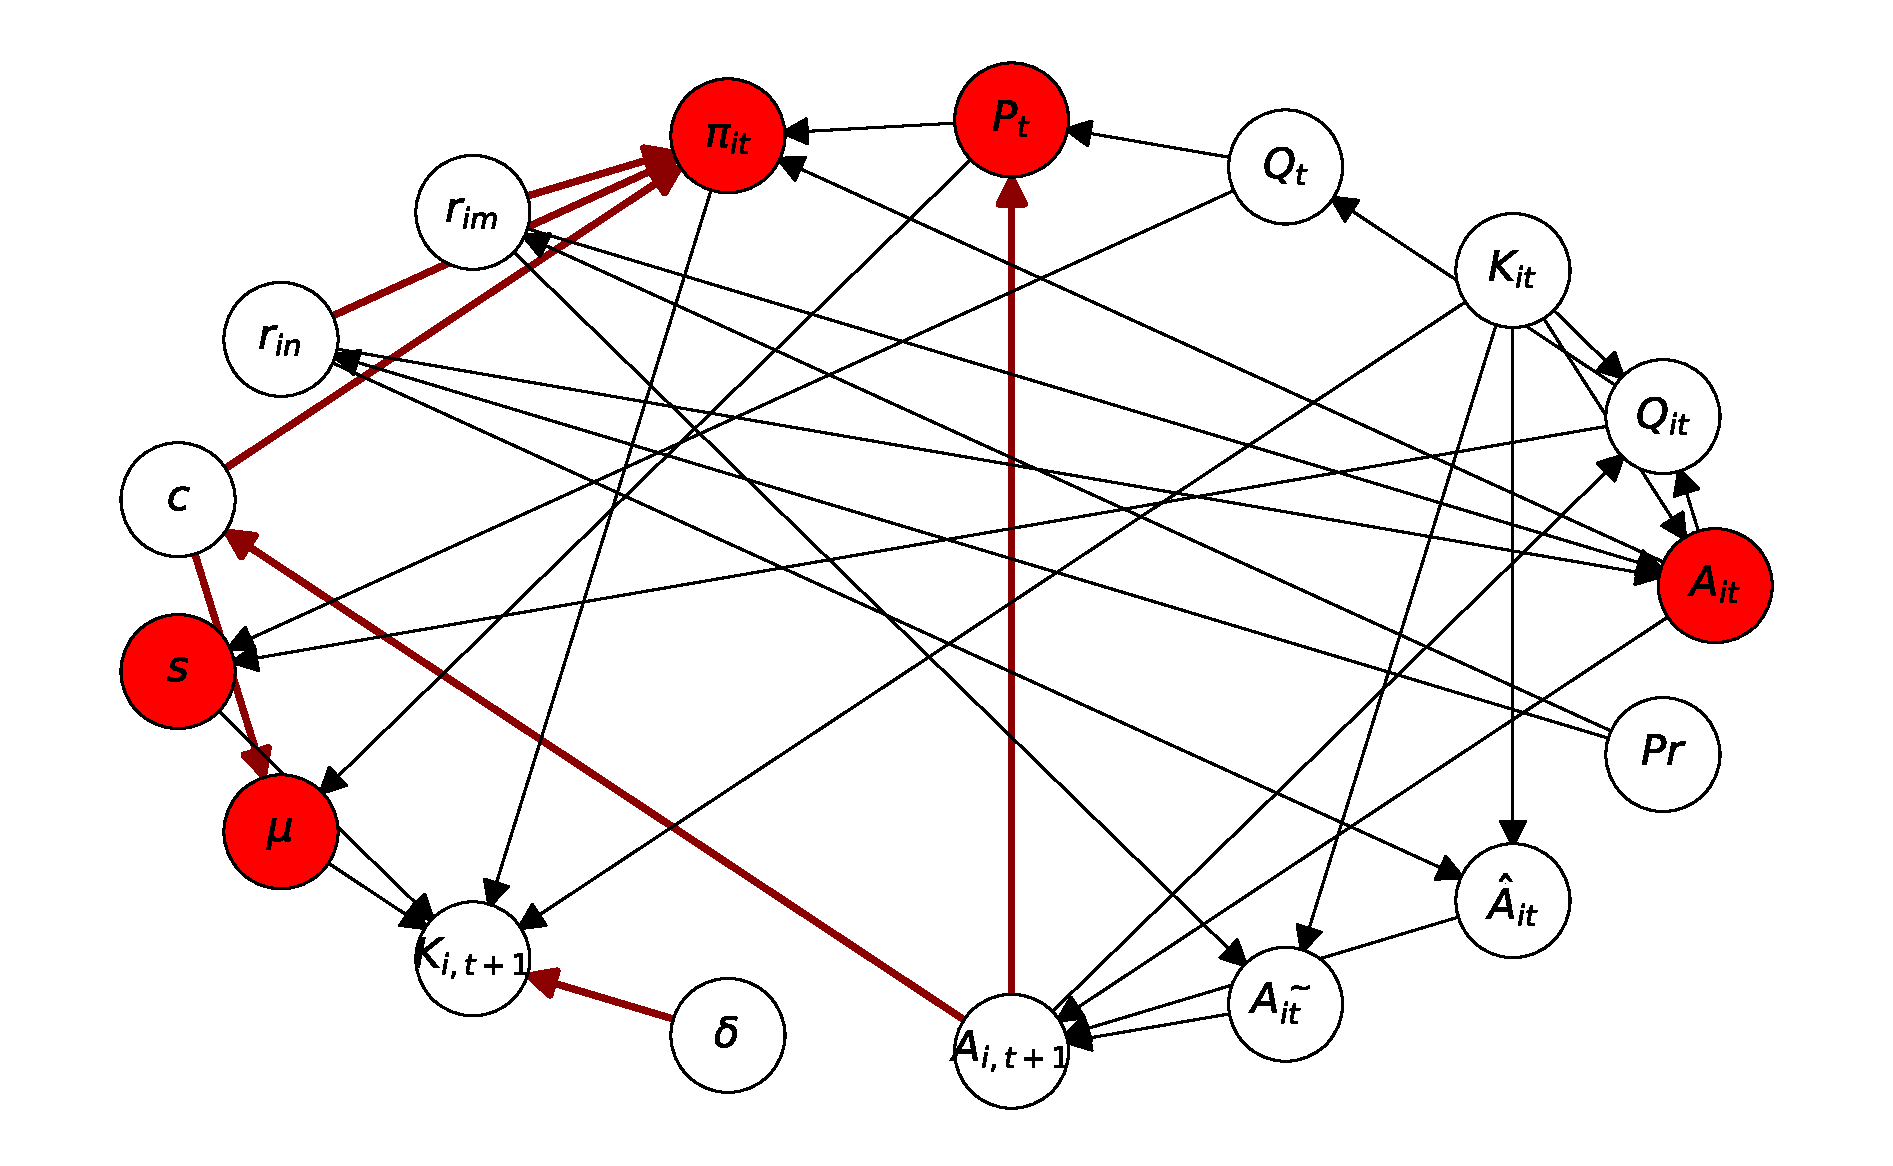
\includegraphics[width=\paperwidth,width=\paperwidth]{modelo.eps}
\end{frame} 

\section{Casos extremos}
\begin{frame}
\frametitle{Casos extremos}
\framesubtitle{Solução analítica}

\begin{table}
\begin{tabular}{c|c|c|c|c|c}
	\hline \hline
	Caso &$r_{in}$&$r_{im}$&$s_i$ & $K_{i,t+1}$ & $E(A_t)$\\ 
	\hline 
	Acomodado & 0 & 0 &$1/N$ & $K_{i,t}$ &\\ 
	\hline 
	Imitadores & 0 & $+$ &  & &\\ 
	\hline 
	Inovadores &  &  &  & &\\ \hline
	Estagnadas &  &  &  &$\delta$ &\\ 
	\hline \hline
\end{tabular} 
\end{table}

\end{frame}

\section{Simulações}


\begin{frame}
\frametitle{Desempenho}
\end{frame}

\begin{frame}
\frametitle{Estrutura de mercado}
\end{frame}

\end{document}